\secnumbersection{PROPUESTA DE SOLUCIÓN}
\label{sec:cap4}

Este capítulo especifica el procedimiento reproducible para estudiar la sensibilidad de \textit{Deep Gravity} frente a la discretización espacial en Santiago. La comparación no presupone que una representación supere a otra: construye las ramas Zona 777, H3-r7 y H3-r8 a partir de una cohorte común, con atributos, particiones y protocolo de evaluación explícitos. Se distinguen un piloto de un día, destinado a comprobar la factibilidad del recorrido, y un experimento mensual agregado, destinado a la evaluación principal. Ambos comparten decisiones estructurales, pero difieren en su escenario, normalización, presupuesto y regla de liberación de prueba.

\subsection{Diseño general y trazabilidad}
\label{sec:diseno_general}

La solución parte de registros DTPM de viajes y etapas, reconstruye extremos válidos a nivel de viaje y aplica una delimitación territorial común. A continuación, dos adaptadores espaciales asignan esos mismos viajes a zonas operativas DTPM o a celdas H3. Cada rama recibe atributos externos, forma pares origen--destino y utiliza la misma familia de modelos y reglas de evaluación. La Figura~\ref{fig:pipeline_santiago} resume esta separación entre núcleo común y adaptadores.

\begin{figure}[htbp]
\centering
\resizebox{\textwidth}{!}{%
\begin{tikzpicture}[
    font=\scriptsize,
    process/.style={draw, rounded corners=2pt, align=center, minimum height=0.8cm, minimum width=2.35cm, inner sep=3pt},
    data/.style={process, fill=blue!8},
    spatial/.style={process, fill=green!9},
    model/.style={process, fill=orange!10},
    arrow/.style={-{Stealth[length=2mm,width=1.4mm]}, thick}
]
    \node[data] (source) {\textbf{DTPM}\\viajes + etapas};
    \node[data, right=0.55cm of source] (canonical) {\textbf{Núcleo canónico}\\unión, extremos y cohorte};
    \node[data, right=0.55cm of canonical] (territory) {\textbf{Dominio común}\\34 comunas y exclusión común};
    \node[spatial, below left=0.95cm and 0.75cm of territory] (zone) {\textbf{Adaptador Zona 777}\\zonas operativas};
    \node[spatial, below right=0.95cm and 0.75cm of territory] (hthree) {\textbf{Adaptador H3}\\r7 y r8};
    \node[model, below=2.35cm of territory] (features) {\textbf{Construcción de atributos}\\Censo 2024 + OSM + distancia};
    \node[model, below=0.75cm of features] (evaluation) {\textbf{Entrenamiento y evaluación}\\particiones por origen, referencias y CPC};

    \draw[arrow] (source) -- (canonical);
    \draw[arrow] (canonical) -- (territory);
    \draw[arrow] (territory.south west) -- (zone.north);
    \draw[arrow] (territory.south east) -- (hthree.north);
    \draw[arrow] (zone.south) |- (features.north west);
    \draw[arrow] (hthree.south) |- (features.north east);
    \draw[arrow] (features.south) -- (evaluation.north);
\end{tikzpicture}
}
\caption{Procedimiento de Santiago: un núcleo común de viajes precede a los adaptadores espaciales y a la evaluación. Fuente: elaboración propia.}
\label{fig:pipeline_santiago}
\end{figure}

La variable de respuesta es el flujo observado agregado entre una unidad de origen $i$ y una unidad de destino $j$. La población censal, el flujo saliente observado, el factor de expansión y los atributos de OSM son magnitudes distintas: el flujo saliente permite reconstruir la masa predicha condicionada al origen, pero no se incorpora como sustituto de población ni como predictor científico.

\subsection{Datos de movilidad y reconstrucción del viaje}
\label{sec:ingesta_datos}

La entrega DTPM disponible comprende 29 fechas, desde el 1 al 29 de noviembre de 2024. Los archivos del día 30 llegaron con errores y se excluyen sin imputación. La unidad observacional utilizada en la comparación es un viaje canónico, no una validación aislada. La unión diaria validada vincula \texttt{viajes.(id\_tarjeta, id\_viaje)} con \texttt{etapas.(id\_etapa, correlativo\_viajes)}. El origen se reconstruye desde la primera etapa y el destino desde una bajada válida de la etapa final; las coordenadas UTM de ambos extremos residen en \texttt{etapas}, no en \texttt{viajes}.

La cohorte primaria exige una secuencia completa y sin duplicados de etapas, numeradas desde uno hasta el número declarado para el viaje. El origen corresponde a la primera etapa y el destino a la bajada de la última; esta debe tener \texttt{tiene\_bajada}=1 y el viaje debe indicar \texttt{ultimaetapaconbajada}=1. Se requieren zonas de origen y destino disponibles y \texttt{factor\_expansion} no negativo. Como control técnico previo al recorte territorial, las coordenadas de ambos extremos deben satisfacer $100.000 \leq X \leq 900.000$ y $5.000.000 \leq Y \leq 10.000.000$, en metros. Estos rangos no definen el área de estudio.

El factor de expansión de \texttt{viajes} es el peso principal para los flujos expandidos; el conteo sin expansión se conserva para el análisis de sensibilidad. La Tabla~\ref{tab:fuentes_variables} distingue procedencia y función de los insumos para evitar confundir pesos, coordenadas y variables explicativas.

\begin{table}[htbp]
\centering
\small
\caption{Fuentes de datos y función de las variables usadas por el procedimiento. Fuente: elaboración propia.}
\label{tab:fuentes_variables}
\begin{tabularx}{\textwidth}{@{}p{2.3cm}p{4.1cm}X@{}}
\toprule
\textbf{Insumo} & \textbf{Contenido o unidad} & \textbf{Uso y regla de trazabilidad} \\
\midrule
\texttt{viajes} DTPM & Identificadores del viaje, zonas consolidadas, secuencia y \texttt{factor\_expansion}. & Aporta la identidad del viaje, las zonas de la rama zonal y la masa expandida. No aporta coordenadas UTM de los extremos. \\
\texttt{etapas} DTPM & Identificadores de etapa y viaje; coordenadas UTM de subida y bajada. & Permite reconstruir origen y destino válidos y asignar H3 tras transformar EPSG:32719 a WGS84. \\
\texttt{ShapeZona} 777 DTPM & Geometría oficial de zonas y sus identificadores. & Sustenta área, centroides y atributos de las zonas; no se fabrican polígonos para IDs sin geometría verificable. \\
Censo 2024 (INE) & Población de manzanas y entidades de la Región Metropolitana. & Se interpola por fracción de área en EPSG:32719 y se expresa por unidad espacial. No equivale a generación observada. \\
OSM Chile 2024-01-01 & Polígonos, vías y puntos del extracto histórico. & Aporta coberturas y densidades utilizadas como atributos territoriales; un cero representa ausencia cartografiada, no prueba de ausencia real. \\
\bottomrule
\end{tabularx}
\end{table}

Para un escenario temporal dado, el flujo expandido se agrega como
\begin{equation}
    T_{ij} = \sum_{v \in \mathcal{V}_{ij}} w_v,
    \label{eq:flujo_expandido}
\end{equation}
donde $\mathcal{V}_{ij}$ reúne los viajes canónicos entre $i$ y $j$, y $w_v$ es el peso expandido del viaje $v$. Las tablas OD operativas conservan, por separado, \texttt{trip\_count} y \texttt{expanded\_mass}; no incluyen identificadores personales.

\subsection{Delimitación territorial y cohorte común}
\label{sec:delimitacion}

El dominio de estudio es el núcleo urbano referencial de 34 comunas. Cada extremo UTM debe estar estrictamente contenido en una de las geometrías comunales DPA 2023 proyectadas a EPSG:32719; los puntos ubicados en un límite se excluyen por la regla \texttt{contains}. El filtro territorial retiene 60.513.881 viajes de la cohorte primaria y 85.777.662,9386 de masa expandida. La Figura~\ref{fig:delimitacion_gran_santiago} documenta esa decisión territorial.

\begin{figure}[htbp]
\centering
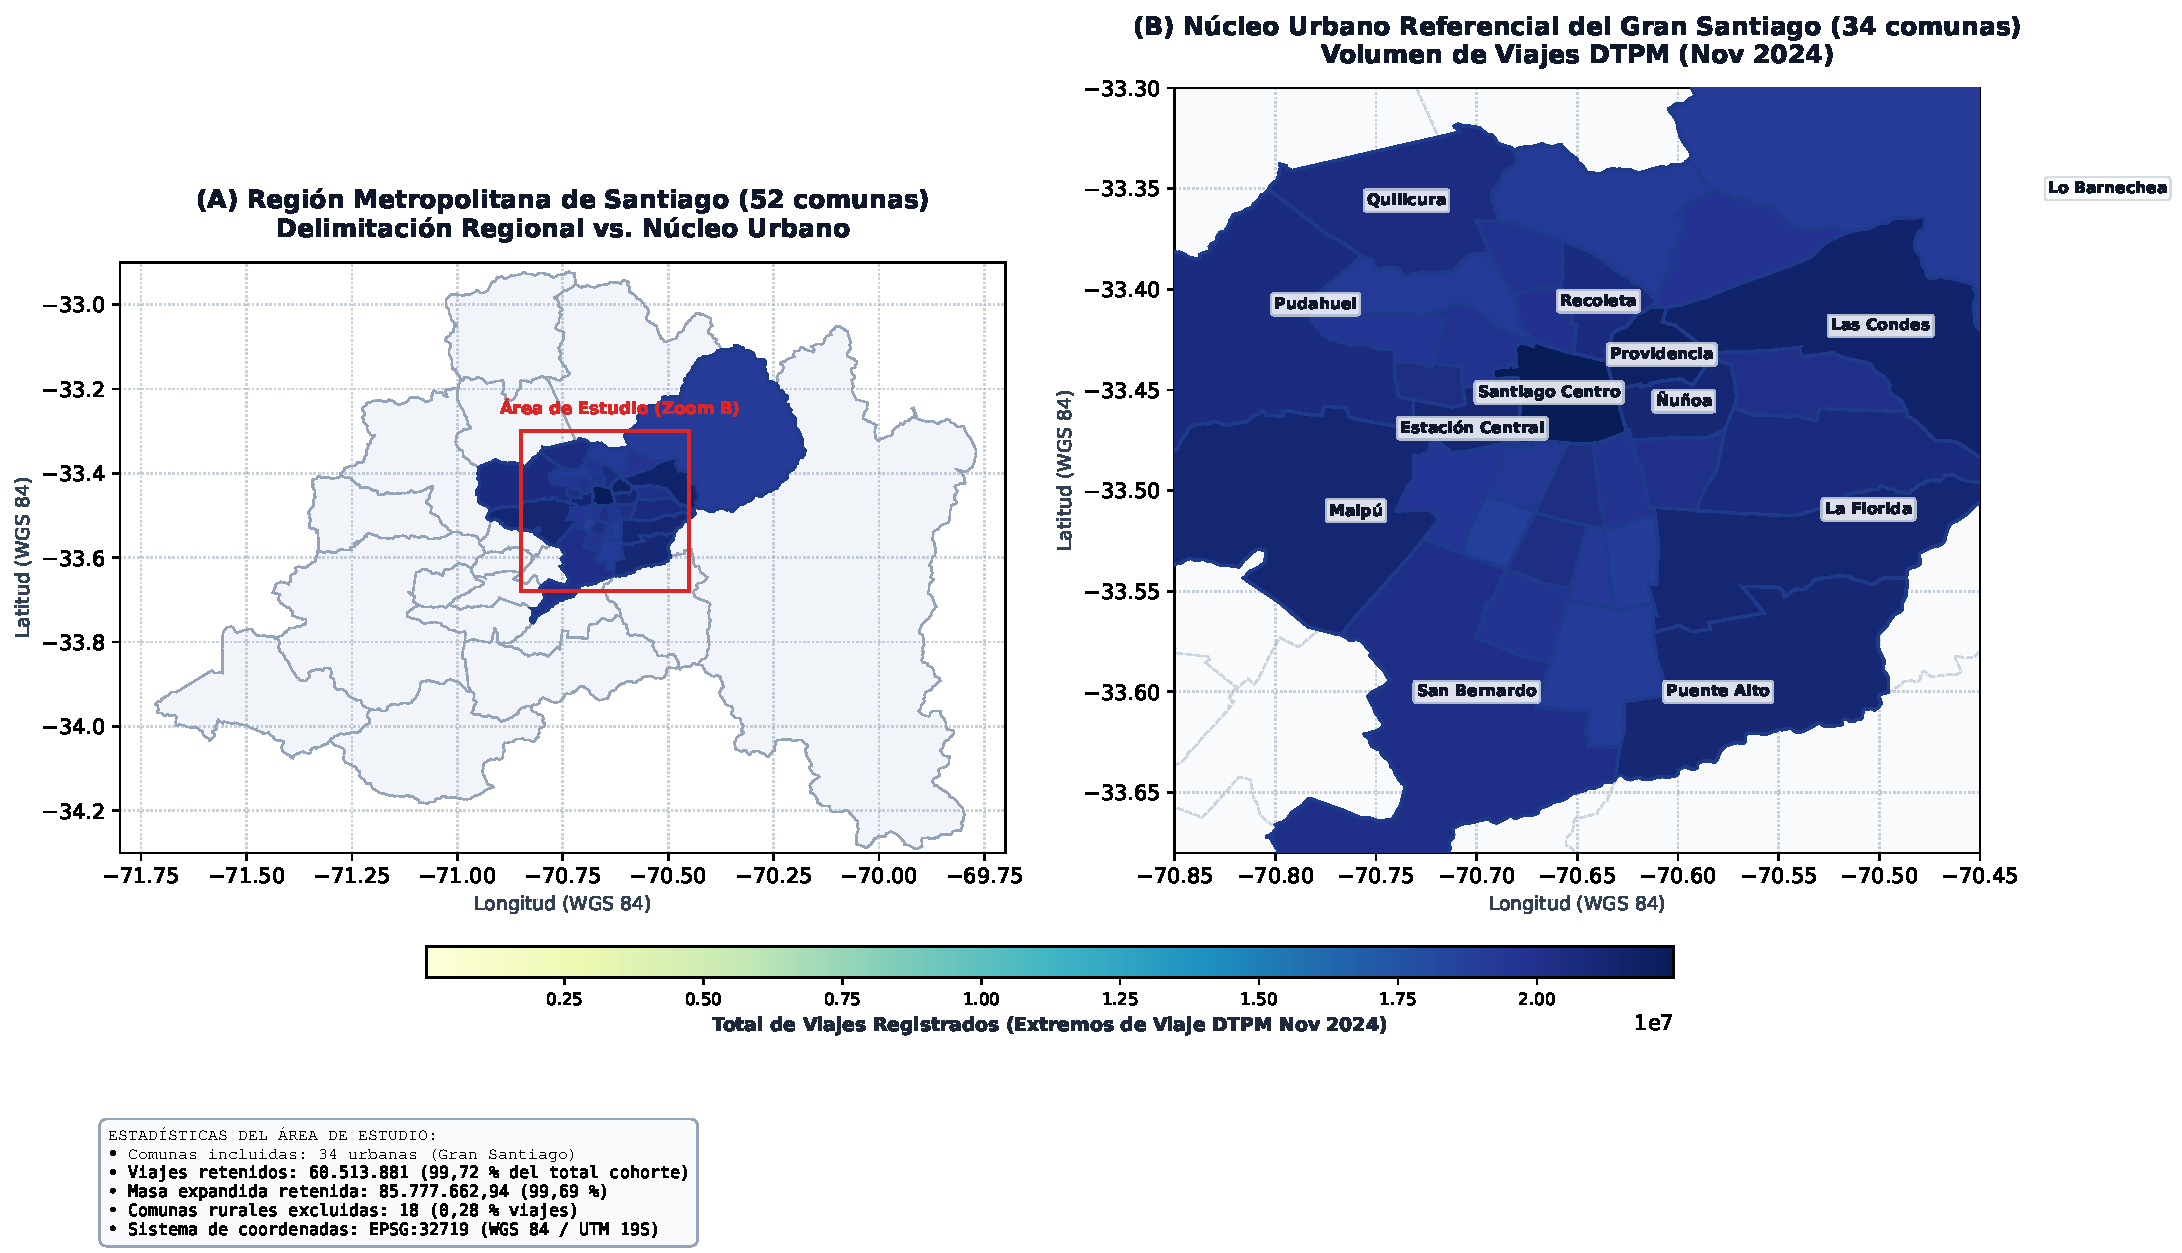
\includegraphics[width=\textwidth]{figures/fig2_delimitacion_gran_santiago_tesis.pdf}
\caption{Delimitación del área de estudio: núcleo urbano referencial de 34 comunas dentro de la Región Metropolitana. Las cifras de la figura corresponden al filtro territorial previo a la exclusión común posterior de tres zonas sin polígono oficial verificable. Fuente: elaboración propia. Los datos territoriales y el procedimiento se describen en esta sección.}
\label{fig:delimitacion_gran_santiago}
\end{figure}

Después del recorte territorial se excluyen, en las tres ramas, los 1.904 viajes que tienen al menos un extremo en las zonas 848, 849 o 852, ya que no disponen de polígono oficial verificable para construir atributos. La cohorte comparativa resultante contiene 60.511.977 viajes y 85.774.522,4070 de masa expandida. Esta exclusión se aplica antes de agregar OD y no se reemplaza mediante geometrías de otra codificación.

La Figura~\ref{fig:serie_diaria_cohorte_final} muestra la cobertura diaria de esta cohorte final. Las 29 fechas disponibles se mantienen con su tipo de día observado; el 30 de noviembre no aparece como cero porque se excluyó por problemas en los archivos de origen.

\begin{figure}[htbp]
\centering
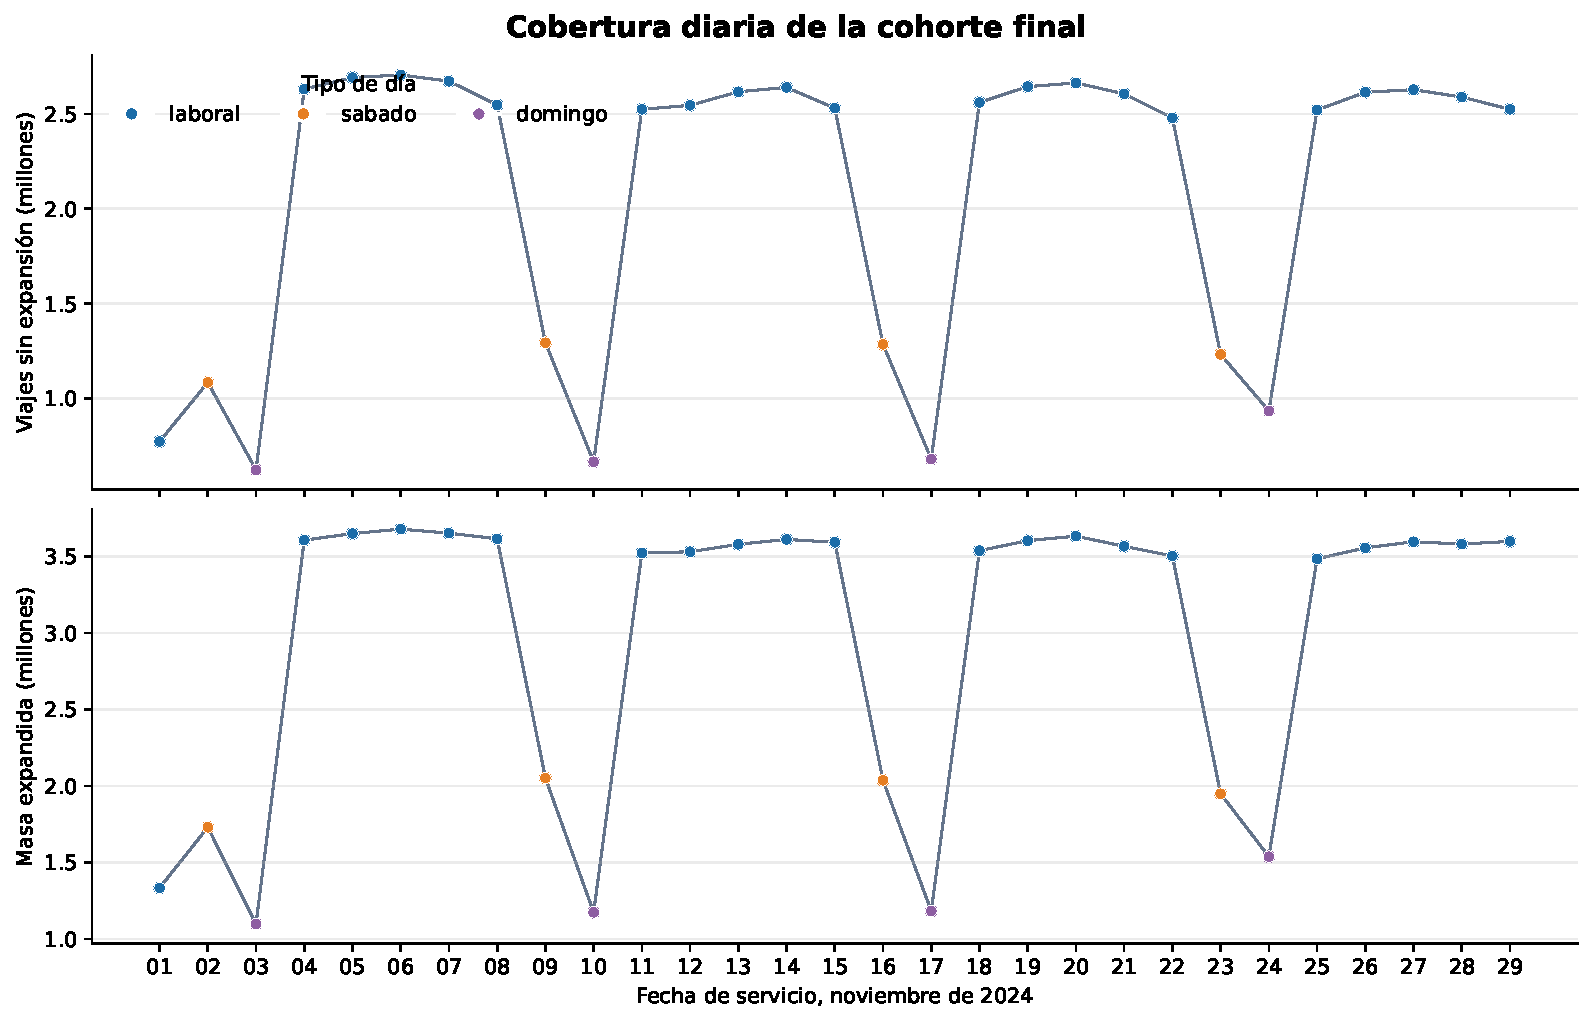
\includegraphics[width=0.93\textwidth]{figures/v05_serie_diaria_cohorte_final.pdf}
\caption{Viajes y masa expandida diarios de la cohorte final. Los puntos distinguen el tipo de día; el OD diario ya está restringido al dominio de 34 comunas y se aplican las exclusiones comunes 848, 849 y 852 en ambos extremos. Se muestran las 29 fechas disponibles, del 1 al 29 de noviembre de 2024; el día 30 no se imputa. Fuente: elaboración propia a partir de los viajes canónicos DTPM.}
\label{fig:serie_diaria_cohorte_final}
\end{figure}

\subsection{Adaptadores espaciales, unidades y \textit{tiles}}
\label{sec:unidades_espaciales}

La rama Zona 777 usa las zonas de origen y destino auditadas en el viaje canónico y la geometría oficial publicada por DTPM. La rama H3 transforma las coordenadas válidas desde EPSG:32719 a WGS84 con \texttt{always\_xy=True} y asigna cada extremo mediante \texttt{latlng\_to\_cell}. La política de borde conserva la celda H3 completa observada: los viajes se recortan por el dominio de estudio, pero las huellas de las celdas no se recortan ni se reparte flujo por superficie.

H3 es un sistema jerárquico de índices geoespaciales. Sus áreas y distancias varían geográficamente, existen pentágonos y la vecindad no puede resumirse como seis vecinos para toda celda. Por ello, H3 no elimina el problema de la unidad espacial modificable (MAUP, por sus siglas en inglés): la comparación trata la discretización espacial como una fuente de sensibilidad empírica. El análisis de factibilidad consideró H3-r3 a H3-r8; H3-r7 y H3-r8 pasaron al piloto junto con Zona 777. La Tabla~\ref{tab:representaciones} presenta las representaciones operativas de la cohorte común, sin inferir superioridad entre ellas.

\begin{table}[htbp]
\centering
\small
\caption{Representaciones espaciales operativas después de la exclusión común. Fuente: elaboración propia.}
\label{tab:representaciones}
\begin{tabularx}{\textwidth}{@{}p{2.1cm}p{2.2cm}p{2.0cm}X@{}}
\toprule
\textbf{Rama} & \textbf{Unidades} & \textbf{Rol} & \textbf{Regla de asignación y alcance} \\
\midrule
Zona 777 & 793 zonas & Referencia zonal & Zonas de origen y destino del viaje canónico; atributos calculados desde la geometría oficial verificable. \\
H3-r7 & 223 celdas & Candidata de escala más agregada & Ambos extremos válidos se asignan directamente a celdas H3; mantiene celdas completas en el borde. \\
H3-r8 & 1.210 celdas & Candidata de mayor detalle & Misma regla de asignación H3 y misma cohorte fuente; su mayor desagregación modifica el soporte OD. \\
\bottomrule
\end{tabularx}
\end{table}

La Figura~\ref{fig:areas_y_soporte_representaciones} complementa esta descripción con las áreas físicas de las unidades y el número de unidades que tienen salida observada en la cohorte completa. Estas diferencias cambian los pares OD evaluables y la masa asignada a prueba; por ello, el CPC se interpreta dentro de cada rama y no como una escala común entre representaciones.

\begin{figure}[htbp]
\centering
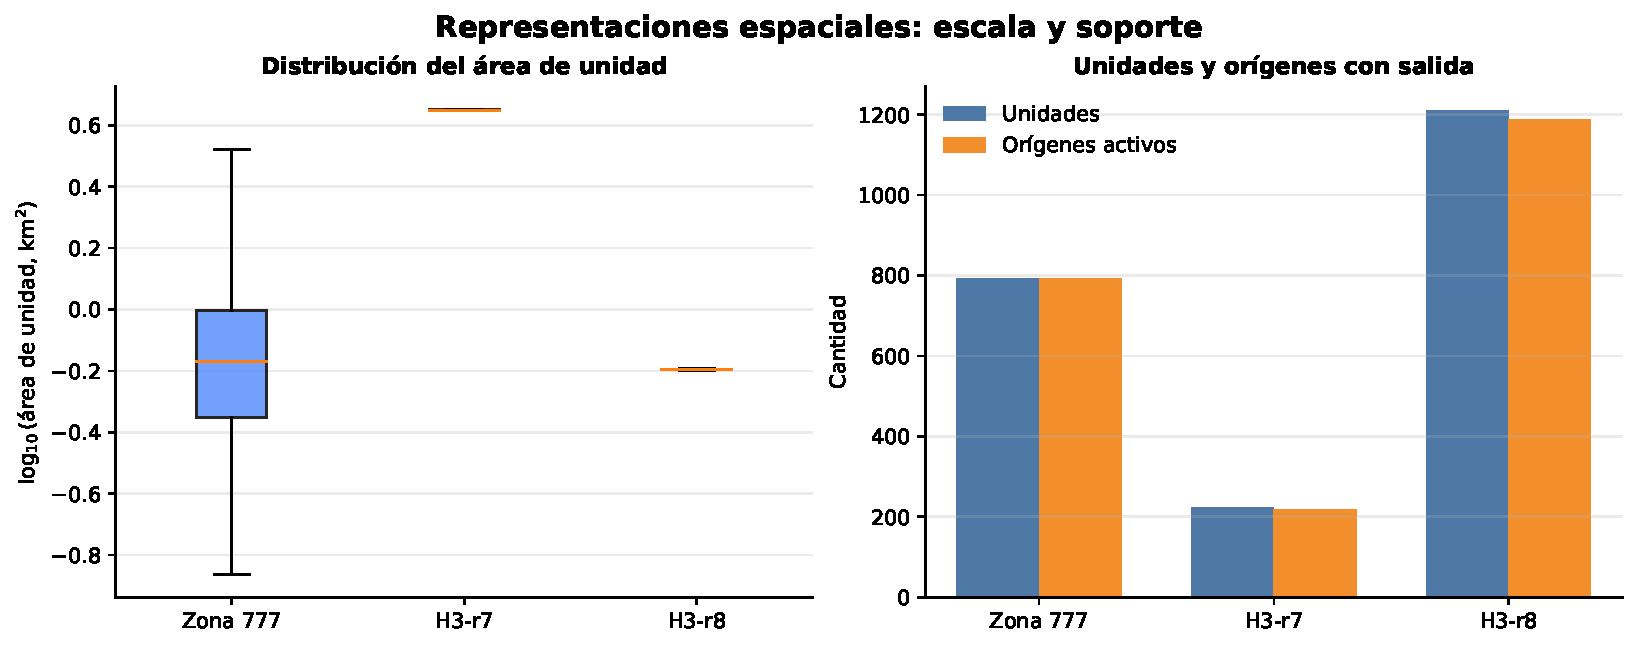
\includegraphics[width=\textwidth]{figures/v07_areas_y_soporte_representaciones.pdf}
\caption{Escalas físicas y soporte de las tres representaciones sobre la misma cohorte final. El panel izquierdo muestra $\log_{10}$ del área de cada unidad en km$^2$; el derecho distingue unidades totales y orígenes con salida observada. La figura no supone igualdad de área ni comparabilidad directa del CPC entre ramas. Fuente: elaboración propia con el contrato territorial y de atributos aprobado y el soporte del experimento mensual.}
\label{fig:areas_y_soporte_representaciones}
\end{figure}

Una zona o celda es una unidad OD. Un \textit{tile} es un bloque mayor, de 15.000 m de lado en EPSG:32719, indexado por $\operatorname{floor}(x/15000)$ y $\operatorname{floor}(y/15000)$. Se fijaron diez \textit{tiles} comunes y una agenda determinista con semilla 20260909: siete para entrenamiento, dos para validación y uno para prueba. La partición se aplica al origen; todos los destinos del dominio de estudio, incluidos los de otros \textit{tiles} o particiones, permanecen candidatos y los flujos cruzados se conservan. La Figura~\ref{fig:objetos_espaciales} distingue estos objetos y evita equiparar un \textit{tile} con una unidad OD.

\begin{figure}[htbp]
\centering
\begin{subfigure}[t]{0.47\textwidth}
\centering
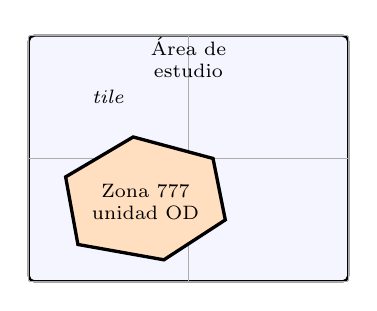
\begin{tikzpicture}[x=0.78cm,y=0.78cm,font=\scriptsize]
    \draw[rounded corners=2pt, thick, fill=blue!4] (0,0) rectangle (5.2,4.0);
    \foreach \x in {0,2.6,5.2} \draw[gray!65] (\x,0) -- (\x,4.0);
    \foreach \y in {0,2,4} \draw[gray!65] (0,\y) -- (5.2,\y);
    \draw[very thick, fill=orange!25] (0.8,0.6) -- (2.2,0.35) -- (3.2,1.0) -- (3.0,2.0) -- (1.7,2.35) -- (0.6,1.7) -- cycle;
    \node[align=center] at (2.6,3.65) {Área de\\estudio};
    \node[align=center] at (1.3,3.0) {\textit{tile}};
    \node[align=center] at (1.9,1.3) {Zona 777\\unidad OD};
\end{tikzpicture}
\caption{Adaptador Zona 777.}
\end{subfigure}
\hfill
\begin{subfigure}[t]{0.47\textwidth}
\centering
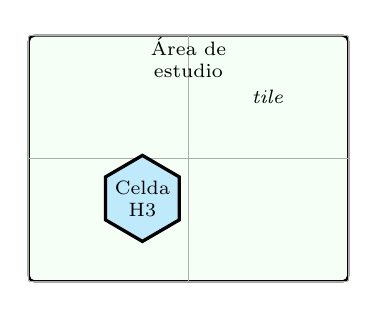
\begin{tikzpicture}[x=0.78cm,y=0.78cm,font=\scriptsize]
    \draw[rounded corners=2pt, thick, fill=green!4] (0,0) rectangle (5.2,4.0);
    \foreach \x in {0,2.6,5.2} \draw[gray!65] (\x,0) -- (\x,4.0);
    \foreach \y in {0,2,4} \draw[gray!65] (0,\y) -- (5.2,\y);
    \draw[very thick, fill=cyan!25] (1.25,1.0) -- (1.85,0.65) -- (2.45,1.0) -- (2.45,1.7) -- (1.85,2.05) -- (1.25,1.7) -- cycle;
    \node[align=center] at (2.6,3.65) {Área de\\estudio};
    \node[align=center] at (3.9,3.0) {\textit{tile}};
    \node[align=center] at (1.85,1.35) {Celda\\H3};
\end{tikzpicture}
\caption{Adaptador H3.}
\end{subfigure}
\caption{Escalas espaciales del procedimiento. Cada rama representa el mismo dominio mediante sus propias unidades OD; el \textit{tile} es un bloque de partición mayor y no reemplaza a una zona o celda. Esquema no a escala. Fuente: elaboración propia.}
\label{fig:objetos_espaciales}
\end{figure}

\subsection{Construcción de atributos y vector de entrada}
\label{sec:features_osm}

La configuración principal utiliza 19 variables por ubicación y, para un par OD, forma un vector de 39 entradas: 19 del origen, 19 del destino y una distancia. Incluye densidad de población censal, cinco coberturas de uso de suelo, tres densidades de longitud vial y cinco familias de servicios, cada una medida mediante densidad de puntos y cobertura de áreas. Se conserva una configuración alternativa para diagnóstico, con 20 variables por ubicación y 41 entradas por par, que no reemplaza la configuración principal del piloto.

\begin{equation}
    \mathbf{x}_{ij} = [\mathbf{a}_{i}^{(19)},\, \mathbf{a}_{j}^{(19)},\, d_{ij}],
    \label{eq:vector_entrada}
\end{equation}
donde $\mathbf{a}_{i}$ y $\mathbf{a}_{j}$ contienen los atributos externos de origen y destino, respectivamente, y $d_{ij}$ es la distancia geodésica calculada desde representantes espaciales en WGS84. La población se interpola desde Censo 2024 a las unidades y se divide por su área para construir la densidad de entrada a la red; no se reemplaza por el flujo saliente observado.

Los polígonos y las vías se recortan y unen dentro de cada categoría antes de calcular cobertura o longitud. Los puntos requieren pertenencia estricta a la unidad. Para densidades y tasas se aplica \texttt{log1p}; las coberturas mantienen su escala física antes de estandarizar. Media y desviación estándar se estiman solo con orígenes activos de entrenamiento de cada rama y escenario, y luego se aplican a validación y prueba. Esta regla impide que el conjunto de prueba intervenga en la normalización.

El piloto ajustó esta transformación con los orígenes activos del 5 de noviembre de 2024. En contraste, el experimento principal recalculó y verificó independientemente la normalización mensual a partir de los atributos sin normalizar y de sus propios orígenes de entrenamiento; no reutilizó los parámetros del piloto. Las variables constantes reciben escala uno. Por tanto, una coincidencia de diccionario de atributos no supone que las transformaciones numéricas de ambos escenarios sean intercambiables.

La Figura~\ref{fig:distribuciones_h3_r7} sitúa las escalas de tres magnitudes en H3-r7 antes de la normalización del modelo. El primer histograma condiciona explícitamente en pares OD positivos; el segundo pondera por masa expandida las distancias geodésicas entre centroides, que no representan recorridos de la red; el tercero usa densidad poblacional física, sin las transformaciones aplicadas a la entrada de la red.

\begin{figure}[htbp]
\centering
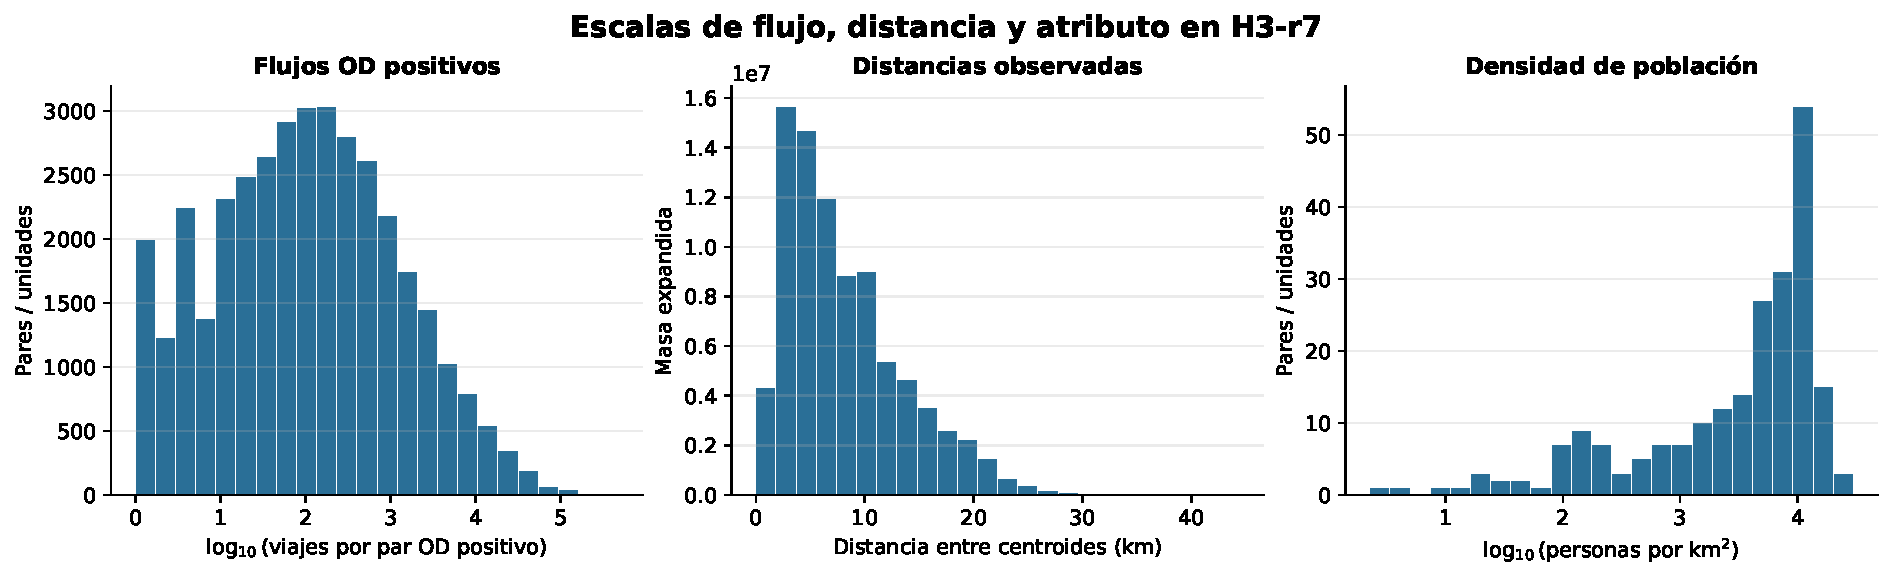
\includegraphics[width=\textwidth]{figures/v06_distribuciones_h3_r7.pdf}
\caption{Escalas de flujo, distancia y densidad poblacional en H3-r7. Los flujos corresponden a pares OD positivos y se expresan en $\log_{10}$ de viajes por par; las distancias entre centroides se agregan con masa expandida; y la densidad poblacional corresponde a personas por km$^2$ antes de la normalización del modelo. Fuente: elaboración propia con la cohorte y los atributos territoriales aprobados.}
\label{fig:distribuciones_h3_r7}
\end{figure}

\subsection{Modelo, muestreo y evaluación}
\label{sec:configuracion_entrenamiento}

\subsubsection{Relación con el modelo gravitatorio}

El \textit{softmax} de una utilidad sistemática $V_{ij}$ define la probabilidad de destino
\begin{equation}
    p_{ij} = \frac{\exp(V_{ij})}{\sum_{k \in \mathcal{D}_i} \exp(V_{ik})},
    \label{eq:logit_dest}
\end{equation}
donde $\mathcal{D}_i$ es el soporte de destinos permitido para el origen $i$. Si $V_{ij}=\beta_1\ln(P_j)+\beta_2\ln(d_{ij})$, el \textit{softmax} induce una forma de potencia $P_j^{\beta_1}d_{ij}^{\beta_2}$; no induce una disuasión exponencial. Una forma gravitatoria exponencial requiere, por ejemplo, una utilidad coherente $V_{ij}=\alpha\ln(P_j)-\beta d_{ij}$ \cite{mcfadden1974conditional,ortuzar2011modelling}.

\textit{Deep Gravity} reemplaza la utilidad lineal por una función no lineal aprendida $f_\theta(\mathbf{x}_{ij})$. El teorema de aproximación universal respalda una capacidad de representación bajo sus supuestos, pero no garantiza que una arquitectura concreta se optimice, generalice o supere a un \textit{baseline} con datos finitos \cite{hornik1991approximation}.

\subsubsection{Arquitectura, soporte y pérdida}

La implementación efectiva conserva 15 capas ocultas: cinco de ancho 256 y diez de ancho 128, con activaciones LeakyReLU. No usa BatchNorm y el \textit{dropout} efectivo es 0,0 en la ruta vigente. La capa final produce un \textit{score} por destino candidato. La arquitectura heredada y la corrida técnica de Nueva York se mantienen como antecedentes de compatibilidad, no como demostración de desempeño científico para Santiago.

El muestreador general permite limitar el número de destinos por origen, sin reposición, y reservar una fracción de candidatos con flujo positivo. Los candidatos restantes se eligen uniformemente entre los disponibles, por lo que pueden incluir otros destinos con flujo positivo. Esa opción no se utilizó en el piloto ni en el experimento mensual: tanto el entrenamiento como la evaluación usaron el soporte completo de destinos de cada representación. Los destinos de todo el dominio metropolitano permanecieron disponibles aunque correspondieran a otro \textit{tile} o partición.

La pérdida es la log-verosimilitud multinomial negativa ponderada por la masa elegida:
\begin{equation}
    \mathcal{L} = -\sum_{i}\sum_{j \in \mathcal{D}_i} y_{ij}\log p_{ij}.
    \label{eq:perdida_multinomial_santiago}
\end{equation}
Para conteos enteros, minimizar esta expresión equivale a maximizar la log-verosimilitud multinomial, salvo constantes independientes del modelo. Con masa expandida fraccionaria, se interpreta como una pérdida multinomial ponderada, con el soporte de destinos y los pesos definidos para el análisis. Su relación con la formulación de entropía de Wilson es conceptual y requiere restricciones adicionales; no se identifica automáticamente con maximizar la entropía de Wilson \cite{wilson1970entropy}.

\subsubsection{Modelos de referencia, particiones y métricas}

Las tres referencias se ajustan solamente con los flujos cuyos orígenes pertenecen a entrenamiento y se evalúan sobre los mismos orígenes, destinos y masa que la red dentro de cada rama. La referencia uniforme asigna $1/|\mathcal{D}|$ a cada destino del soporte. La referencia de atracción usa la masa expandida recibida durante entrenamiento:
\begin{equation}
    \widehat y_{ij}=O_i\,
    \frac{A_j^{\mathrm{train}}+\lambda}
    {\sum_{k\in\mathcal{D}}A_k^{\mathrm{train}}+\lambda|\mathcal{D}|},
    \qquad \lambda=1.
    \label{eq:baseline_atraccion}
\end{equation}
donde $A_j^{\mathrm{train}}$ es la masa que llega a $j$ desde los orígenes de entrenamiento, $\mathcal{D}$ es el soporte completo de destinos de la rama y $O_i$ es el flujo saliente observado del origen que se evalúa. El pseudoconteo $\lambda$ corresponde a una unidad de masa por destino. Esta referencia distribuye una salida observada; no es población, ni un atributo de la red, ni una estimación de la generación de viajes.

En el modelo gravitatorio exponencial, la utilidad se calcula como
\begin{equation}
    V_{ij}=\alpha\ln(1+P_j)+\beta d_{ij},\qquad \alpha\geq0,\quad\beta\leq0,
    \label{eq:baseline_exponencial}
\end{equation}
donde $P_j$ es la población total interpolada, recuperada multiplicando la densidad censal por el área de la unidad, y $d_{ij}$ es la distancia esférica en kilómetros. Los parámetros se ajustan exclusivamente con los flujos de entrenamiento mediante una pérdida multinomial ponderada y L-BFGS-B, inicializado en $(1,-0{,}1)$, con un máximo de 500 iteraciones, $\textit{ftol}=10^{-12}$ y $\textit{gtol}=10^{-8}$; se imponen $\alpha\geq0$ y $\beta\leq0$. Esta variable del modelo de referencia se distingue de la densidad de población transformada y estandarizada que recibe la red. La distancia intrazonal o intracelda es cero, valor admisible en la disuasión exponencial.

El piloto verificó la comparación contra estas tres referencias en el mismo soporte de cada rama. El \textit{checkpoint} se selecciona por CPC de validación; la prueba se ejecuta después y no ajusta parámetros. La configuración del piloto usa RMSprop, tasa de aprendizaje $5\times10^{-6}$, momento 0,9, lotes de ocho orígenes y 15 épocas. Estos valores son una configuración de piloto registrada, no una selección definitiva de hiperparámetros para el experimento mensual.

La métrica principal es
\begin{equation}
    \mathrm{CPC}=\frac{2\sum_{ij}\min(T_{ij},\widehat{T}_{ij})}{\sum_{ij}T_{ij}+\sum_{ij}\widehat{T}_{ij}}.
    \label{eq:cpc_santiago}
\end{equation}
Se guardan numerador y ambas masas por origen para agregar CPC global y por \textit{tile} sobre el mismo soporte. Las medias por origen, por todos los \textit{tiles} y condicionadas a CPC positivo se reportan separadamente. El piloto de Santiago confirma que el procedimiento se puede ejecutar y repetir con tres semillas, pero una comparación directa de CPC entre resoluciones no demuestra por sí sola superioridad de H3: cambian la agregación, los representantes espaciales y la masa de prueba entre ramas.

\subsubsection{Piloto y experimento mensual}

El piloto utilizó el martes 5 de noviembre de 2024. Incluyó diagnósticos en una muestra, en el día completo y en tres ventanas horarias, y nueve corridas estables del día completo: tres ramas y las semillas 20260909, 20260910 y 20260911. Cada corrida estable se entrenó durante 15 épocas; el mejor \textit{checkpoint} de validación se conservó y se evaluó posteriormente en prueba. Las ventanas y el número de épocas sirvieron para comprobar la factibilidad y estabilidad iniciales, no para establecer convergencia, ajustar hiperparámetros ni generalizar el comportamiento de un día al período mensual.

El experimento principal agrega las 29 fechas disponibles entre el 1 y el 29 de noviembre de 2024; el día 30 se excluye por problemas en los archivos y no se imputa. Se entrenaron nueve modelos desde inicializaciones nuevas: las tres ramas y las mismas tres semillas. La red, el soporte completo y la pérdida fueron los descritos antes. El optimizador fue RMSprop con tasa $5\times10^{-6}$, momento 0,9, $\alpha=0{,}99$, $\epsilon=10^{-8}$, sin decaimiento de pesos ni centrado; se usaron lotes de ocho orígenes en orden estable y sin barajado. Las corridas se ejecutaron secuencialmente en CPU con cuatro hilos. Cada época evaluó todos los orígenes de validación.

La selección del \textit{checkpoint} y la parada anticipada obedecieron a reglas diferentes. Se conservó el \textit{checkpoint} con el mayor CPC global de validación entre todas las épocas ejecutadas y, ante un empate exacto, el primero. Para la parada, la primera época de validación inicializó una referencia significativa; esta se actualizó solo si el CPC posterior era estrictamente mayor que la referencia más $0{,}0001$. Tras un mínimo de 50 épocas, la corrida se detenía cuando acumulaba 30 épocas sin esa mejora significativa. El límite inicial fue 200 épocas: alcanzarlo sin meseta no se interpretaba como convergencia ni autorizaba una extensión automática.

Dos corridas alcanzaron dicho límite y recibieron una autorización previa a la prueba para continuar, sin reinicializar ni alterar datos, particiones, arquitectura, optimizador, métrica o regla de selección. La continuación elevó el máximo a 300 épocas para Zona 777 con semilla 20260909 y H3-r8 con semilla 20260910. Ambas cerraron posteriormente por la misma regla de meseta, en las épocas 226 y 218, respectivamente; sus \textit{checkpoints} seleccionados permanecieron en las épocas 196 y 188. Las demás corridas cerraron con la configuración inicial. La prueba se liberó una sola vez después de congelar las fuentes, las decisiones de validación y los \textit{checkpoints} seleccionados; no intervino en la elección de época, semilla, parámetros o representación.

Como análisis de sensibilidad de la evaluación, las probabilidades ya congeladas se aplicaron también a los conteos OD sin expansión y se reescalaron por el flujo saliente no expandido de cada origen. El CPC resultante es secundario: no implica reentrenamiento sin pesos, nueva selección ni un nuevo ajuste de los modelos de referencia, cuyos parámetros se obtuvieron con la masa expandida.

\subsection{Análisis complementario de atribuciones predictivas}

Después de congelar los modelos mensuales se evaluó la viabilidad de explicar la log-probabilidad condicional de un destino dentro del soporte completo de cada origen. Los representantes se escogieron por la mediana del CPC de validación de cada rama, sin usar el CPC de prueba ni la apariencia de una atribución. Las referencias se construyeron exclusivamente con orígenes de entrenamiento de la rama correspondiente; la función explicada, la muestra y los controles se fijaron antes de cada ejecución. Se ensayaron gradientes integrados con cuadratura Gauss--Legendre \cite{sundararajan2017axiomatic}, SHAP por permutaciones agrupadas y valores de Shapley exactos para grupos jerárquicos \cite{lundberg2017shap}. En todos los casos las atribuciones se definieron como sensibilidad predictiva dependiente de la referencia, no como efectos causales.

Las tres aproximaciones se evaluaron contra controles de integridad, coincidencia entre el adaptador y la salida del modelo, finitud, convergencia o eficiencia según el método, repetibilidad y estabilidad frente a fondos independientes. Los gradientes integrados no acreditaron completitud para una consulta crítica aun con 4.096 nodos. El método por permutaciones no acreditó estabilidad entre fondos en dos de tres semillas de su primera consulta obligatoria. El método exacto jerárquico acreditó una primera consulta a 24 fondos, pero otra consulta crítica no acreditó la estabilidad de los tres supergrupos a 24 ni a 48 fondos. En consecuencia, ninguna aproximación superó todos los controles requeridos para publicar atribuciones. No se presentan rankings, atribuciones, figuras SHAP ni casos locales; los registros técnicos se conservan como respaldo reproducible y el desenlace se desarrolla en el Capítulo~5.

\subsection{Reproducibilidad, alcances y limitaciones}
\label{sec:alcances}

Cada ejecución conserva configuración efectiva, semillas, versiones, hashes de entradas y código, particiones, métricas y \textit{checkpoint} en un directorio exclusivo. Los productos de datos, las especificaciones de procesamiento y los registros de ejecución permiten verificar la conservación de masa y reconstruir la procedencia de cada corrida. La prueba espacial se mantiene reservada durante la selección; el conjunto de prueba no participa en la normalización ni en el ajuste de hiperparámetros.

El alcance se limita a la movilidad observable en DTPM durante las 29 fechas disponibles de noviembre de 2024 y al dominio de estudio de 34 comunas. No representa todos los modos urbanos, no predice la generación total de viajes por origen ni fechas futuras. El piloto no acredita por sí mismo generalización temporal al período mensual. A su vez, el agregado mensual incluye el 5 de noviembre y reutiliza la misma geografía de prueba, por lo que no constituye una prueba enteramente nueva e independiente del piloto. Las tres semillas caracterizan variación de inicialización bajo una sola partición espacial, no incertidumbre espacial o poblacional. La instantánea OSM antecede a los viajes y su cobertura no equivale a presencia real de servicios; la interpolación areal del Censo 2024 supone distribución uniforme dentro de cada geometría censal. Además, la exclusión de las zonas sin polígono, la decisión de discretización y las diferencias de agregación espacial condicionan toda interpretación comparativa.

El resultado del análisis complementario de explicabilidad limita la interpretación de las características territoriales: bajo las configuraciones ensayadas no fue posible obtener atribuciones suficientemente estables para una interpretación sustantiva. Esta limitación no altera las métricas predictivas ni las comparaciones con referencias, que se fundamentan en su propio protocolo de evaluación.
